\documentclass{article}
\usepackage[margin=0.6in]{geometry}
\usepackage{amsmath}
\usepackage{amssymb}
\usepackage{bookmark}
\usepackage{graphicx}
\usepackage{float}
\usepackage{hyperref}

\title{Report for Assignment - 2 \\ CS6370: Information Retrieval}
\author{
Harsh Agarwal\\\texttt{CS15BTECH11019}
\and
Sukrut Rao\\\texttt{CS15BTECH11036}
\and
Vishwak Srinivasan\\\texttt{CS15BTECH11043}
}
\date{}

\begin{document}
\maketitle

\section{Introduction}
\begin{flushleft}
This assignment is an exercise in parsing and processing a text. Once processed the assignment expects us to use certain metrics and obtain top-20 words and the note the distribution of the metric.
\end{flushleft}

\section{Processing}
\subsection{Crawling and Parsing HTML}
\begin{flushleft}
The first step is to get the book in HTML form, given its URL, and to split it into text files for individual chapters. This involves fetching the book, extracting the text content, and parsing it to remove irrelevant text, such as metadata. Then, the book is separated into chapters. This separation is dependent on the pattern in which chapters are demarcated in each book, and would vary from book to book. Hence, our script for parsing the book assumes a specific book - \textit{\href{https://www.gutenberg.org/files/1342/1342-h/1342-h.htm}{Pride and Prejudice}} by Jane Austen, from \href{https://www.gutenberg.org}{Project Gutenberg}. However, many books on Project Gutenberg are found in very similar formats, and it should be easy to modify the script to cater to other books. The code for fetching, parsing, separating the book into chapters, and saving each chapter in a separate text file can be found in \verb|parse_book.py|.

The procedure is as follows:
\begin{enumerate}
\item The book in HTML form is fetched from the URL specified. Using the \verb|BeautifulSoup| package, it is converted entirely to text.
\item Using regular expressions, points of demarcation of individual chapters are found. Similarly, the point demarcating the end of the book is also found.
\item The book text is split into individual chapters. Each chapter is saved in the separate text file in the output path specified.
\item The file name for each chapter includes the URL where the book was obtained from. However, forward slashes (\verb|/|) are replaced with the \verb|#| character.
\end{enumerate}

\subsubsection*{Notes}
\begin{enumerate}
\item To use the script for other Project Gutenberg books, the regular experssions for finding the chapter demarcator and the demarcator for the end of the book may have to be modified.
\item Usage instructions in further detail can be found in the \verb|README.md| file.
\end{enumerate}
\end{flushleft}
\newpage

\subsection{Text processing of the datasets}
\begin{flushleft}
The following are the steps for processing:
\begin{enumerate}
\item Case Folding - convert all documents to lower case. For example: ``I didn't create Atlantis'' becomes ``i didn't create atlantis''.
\item Removal of special characters and digits - all special characters (quotes, commas, apostrophes, fullstops, etc.) and digits (0 to 9) were removed. This meant that at the end of this step we had nothing but raw text composed of alphabets alone. For example: ``don't'' becomes ``dont'' and ``ariane-5'' becomes ``ariane''.
\item Removal of stop words - using \texttt{NLTK}'s corpus of stop words, this was easy.
\item Lemmatization - for this we used \texttt{NLTK}'s \texttt{WordNetLemmatizer}.
\end{enumerate}
\end{flushleft}
\newpage

\section{Plots, Top 20 words and Observations - Chapter Wise}
\subsection{Plots}
\begin{flushleft}
The following are the frequency distribution plots obtained for 10 out of 62 chapters. 
\begin{figure}[H]
\begin{minipage}{0.42\linewidth}
\centering
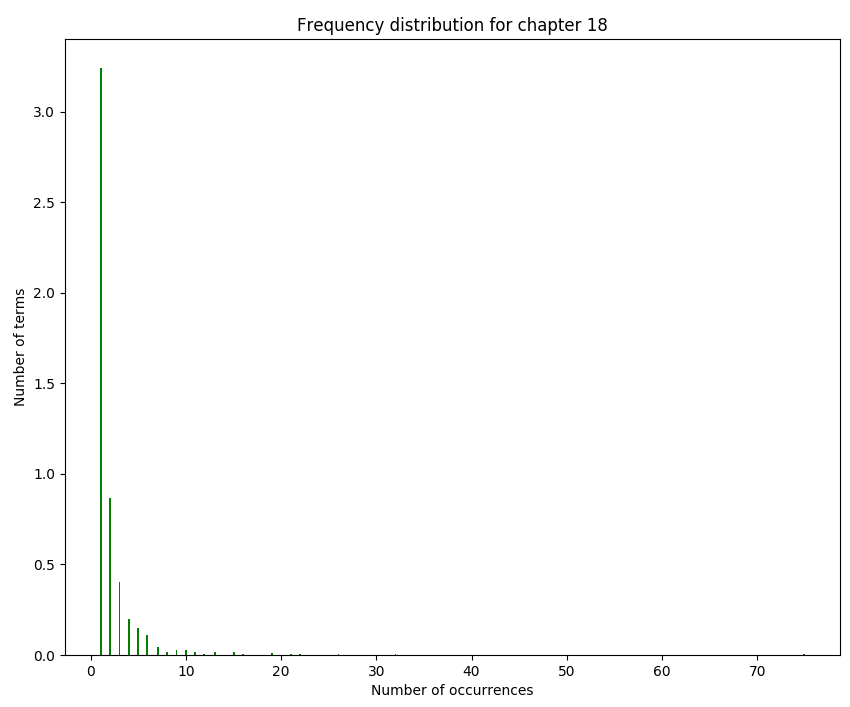
\includegraphics[width=0.65\textwidth]{./images/1-chapter_wise-frequency.png}
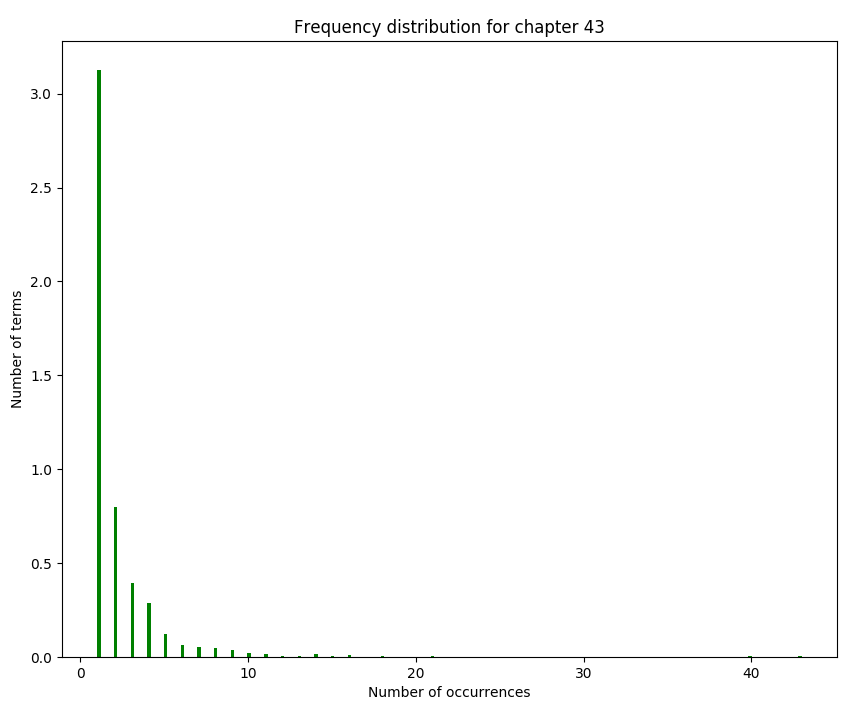
\includegraphics[width=0.65\textwidth]{./images/2-chapter_wise-frequency.png}
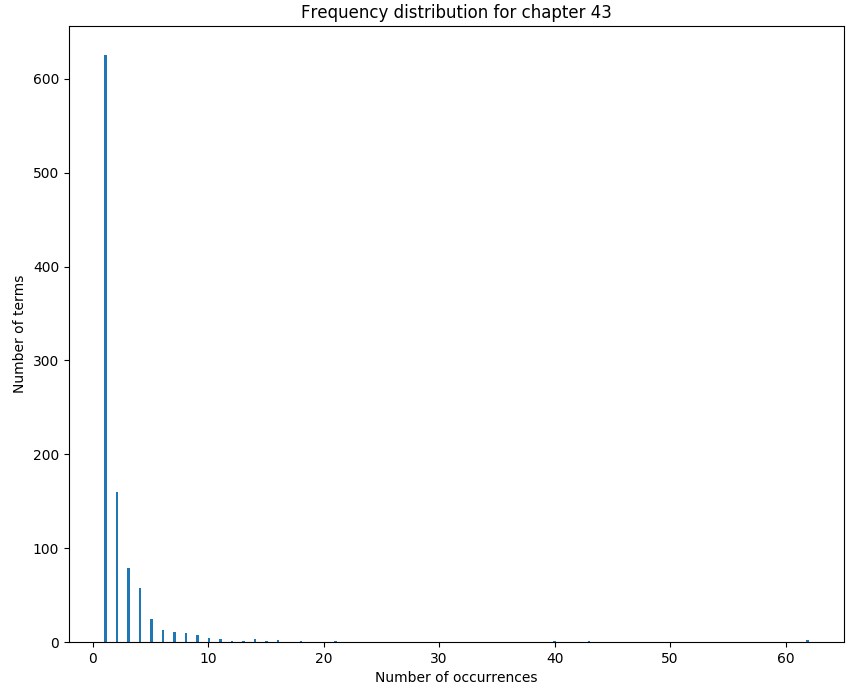
\includegraphics[width=0.65\textwidth]{./images/3-chapter_wise-frequency.png}
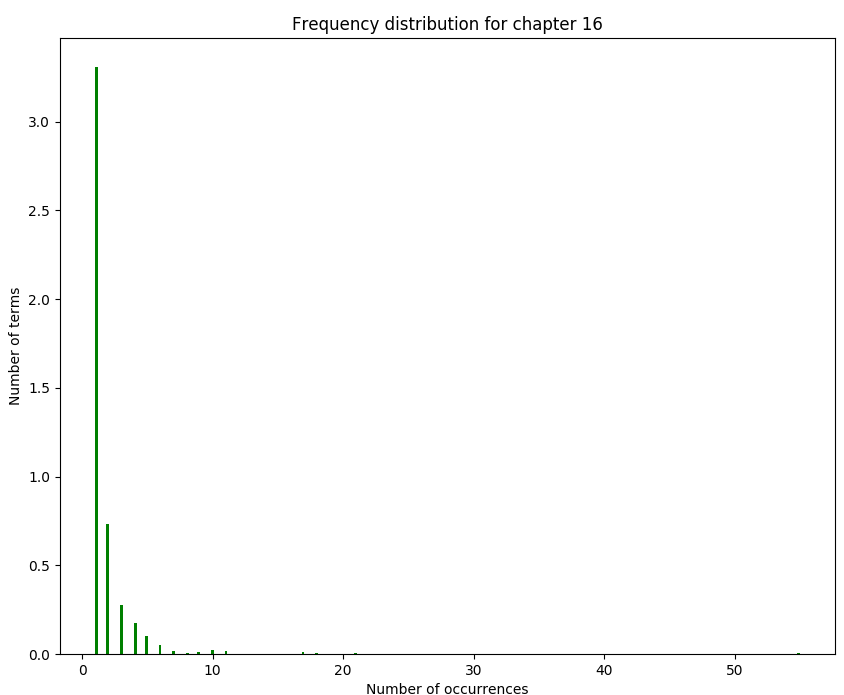
\includegraphics[width=0.65\textwidth]{./images/4-chapter_wise-frequency.png}
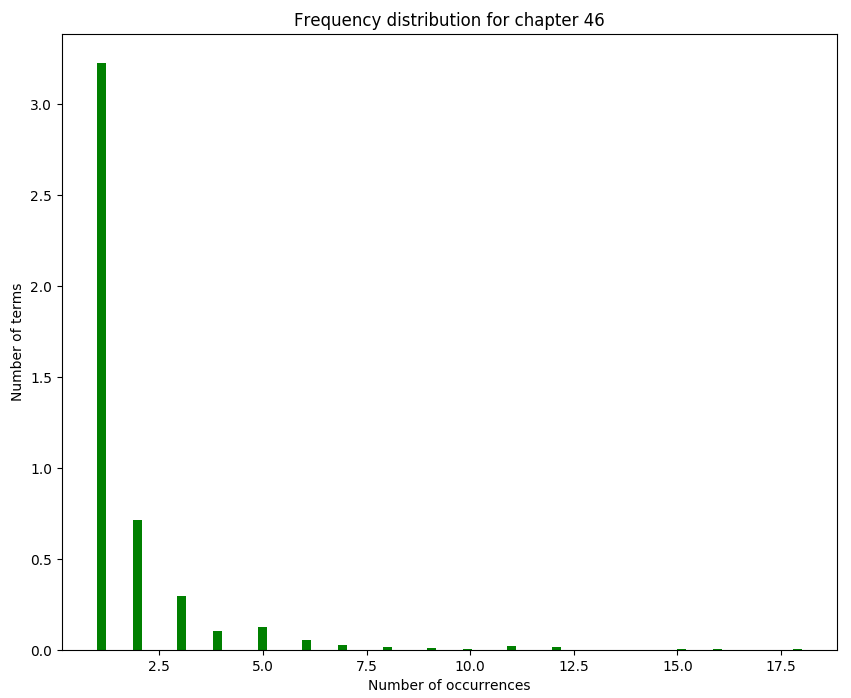
\includegraphics[width=0.65\textwidth]{./images/5-chapter_wise-frequency.png}
\end{minipage}
\hfill
\begin{minipage}{0.42\linewidth}
\centering
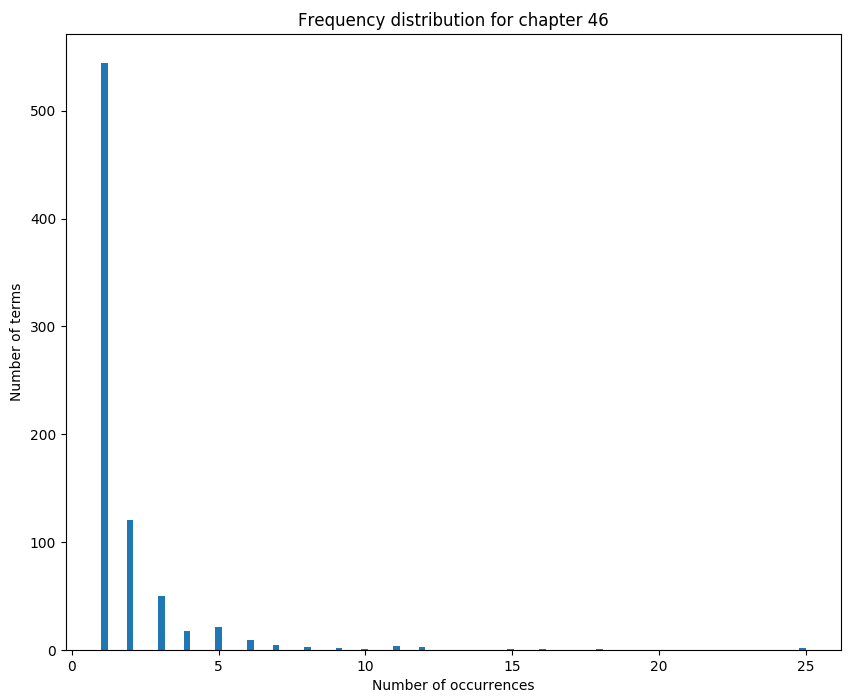
\includegraphics[width=0.65\textwidth]{./images/6-chapter_wise-frequency.png}
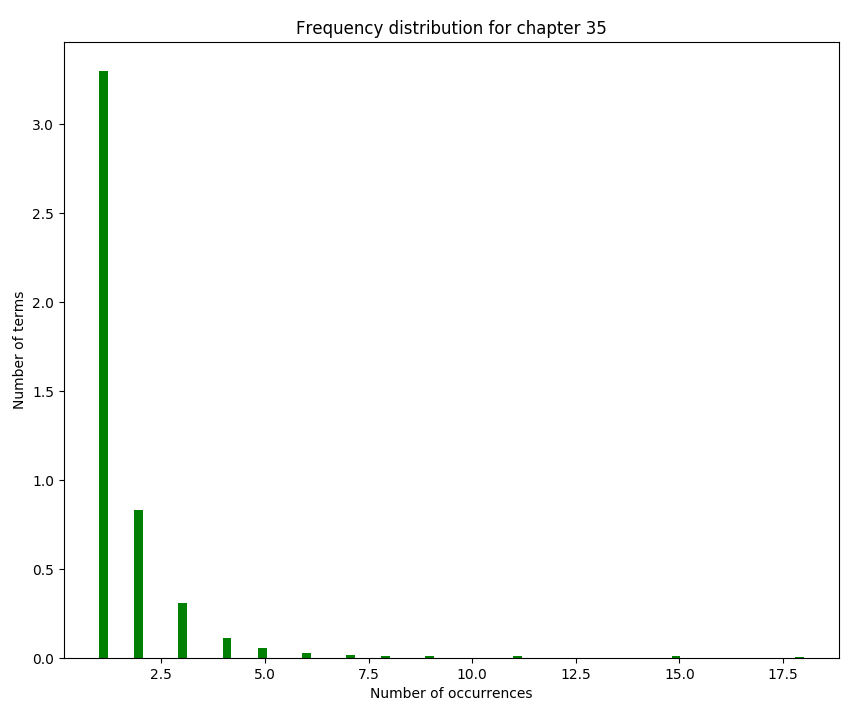
\includegraphics[width=0.65\textwidth]{./images/7-chapter_wise-frequency.png}
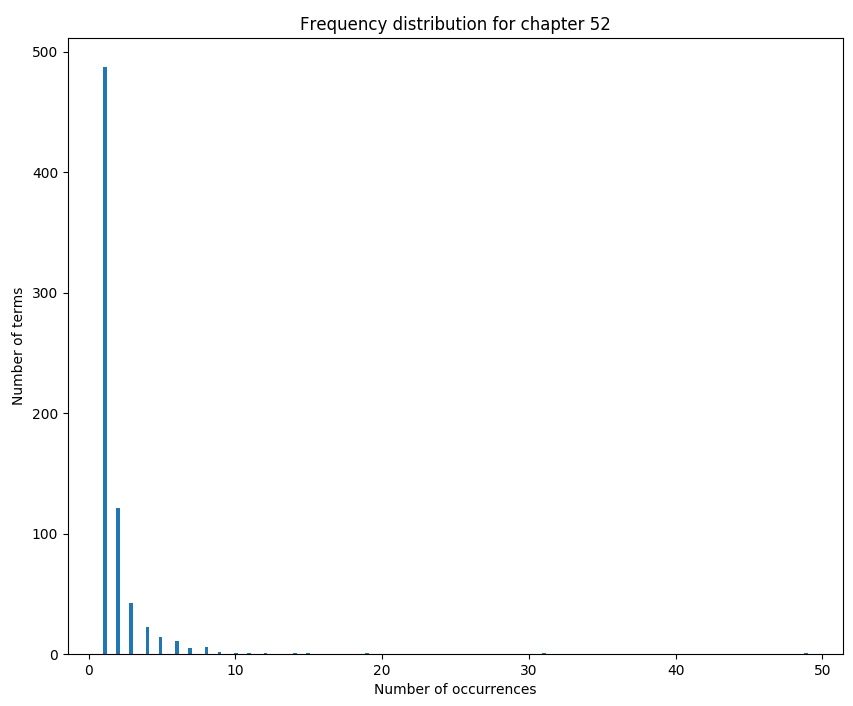
\includegraphics[width=0.65\textwidth]{./images/8-chapter_wise-frequency.png}
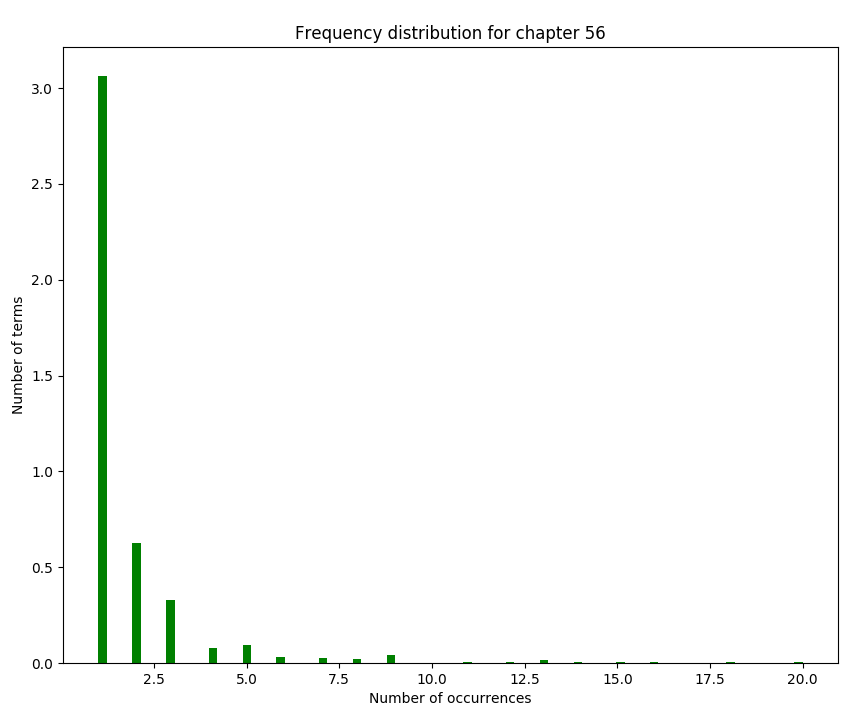
\includegraphics[width=0.65\textwidth]{./images/9-chapter_wise-frequency.png}
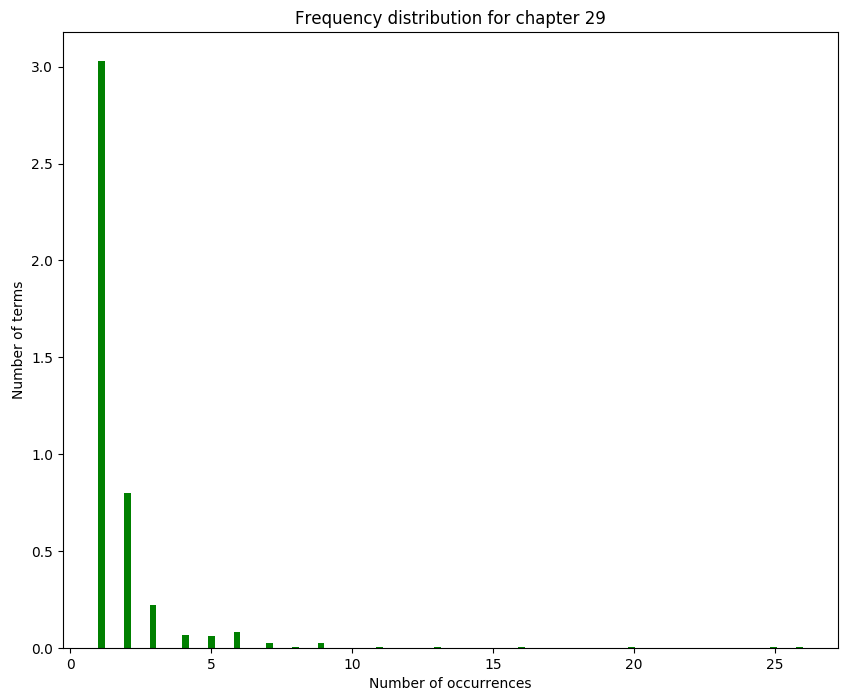
\includegraphics[width=0.65\textwidth]{./images/10-chapter_wise-frequency.png}
\end{minipage}
\caption{Each plot from top to bottom represents a different chapter.\newline{}These are (ordered from top to bottom): 62, 18, 43, 47, 16, 46, 53, 52, 35, 56. These chapters are the chapters with the largest number of terms in them.}
\end{figure}
\end{flushleft}

\subsection{Top 20 words}
\begin{flushleft}
The top 20 words (based on frequency) obtained for 10 chapters are as follows:
\begin{center}
\begin{tabular}{|p{0.08\textwidth}|p{0.37\textwidth}||p{0.08\textwidth}|p{0.37\textwidth}|}
\hline
Chapter Number & Top 20 Words & Chapter Number & Top 20 Words \\
\hline
\hline
18 & mr, darcy, elizabeth, could, said, bingley, though, wickham, sister, say, lady, much, must, may, would, time, collins, dance, however, make &
43 & mr, elizabeth, could, gardiner, said, might, master, thought, darcy, much, every, know, room, aunt, time, good, little, seen, uncle, manner \\ 
\hline
47 & could, know, elizabeth, lydia, well, mr, jane, give, would, think, must, might, u, much, wickham, one, hope, every, colonel, make  &
16 & mr, darcy, elizabeth, wickham, could, said, lady, man, manner, father, much, pride, collins, phillips, nothing, catherine, believe, know, thought, must \\
\hline
46 & could, mr, lydia, elizabeth, must, would, though, letter, nothing, one, know, darcy, u, first, colonel, never, father, gardiner, well, ill &
53 & mr, said, know, could, elizabeth, bennet, bingley, sister, jane, come, see, without, one, much, daughter, looked, never, must, soon, time \\
\hline
35 & mr, sister, could, father,  wickam, must, would, last, soon, letter, year, one, though, every, shall, may, feeling, manner, night, two  &
52 & would, mr, wickham, could, must, uncle, darcy, time, sister, lydia, every, done, much, know, though, soon, town, never, u, letter  \\
\hline
56 & elizabeth, bennet, lady, miss, catherine, would, mr, ladyship, nephew, know, shall, said, make, must, say, mother, family, well, moment, though &
29 & lady, mr, catherine, elizabeth, could, much, sir, said, miss, ladyship, governess, one, de, without, manner, william, daughter, sister, mother \\
\hline
\end{tabular}
\end{center}
\end{flushleft}

\subsection{Observations}
Most of these plots follow an exponential distribution. In all of the chapters, the title of the person seems to occur more than others. There are a lot of proper nouns (names of people and places), and few adjectives and fewer verbs.

\section{Plots, Top 20 words and Observations - Complete Book}
\subsection{Metric: Frequency}
\subsubsection{Distribution Plot}
\begin{flushleft}
\begin{figure}[H]
\centering
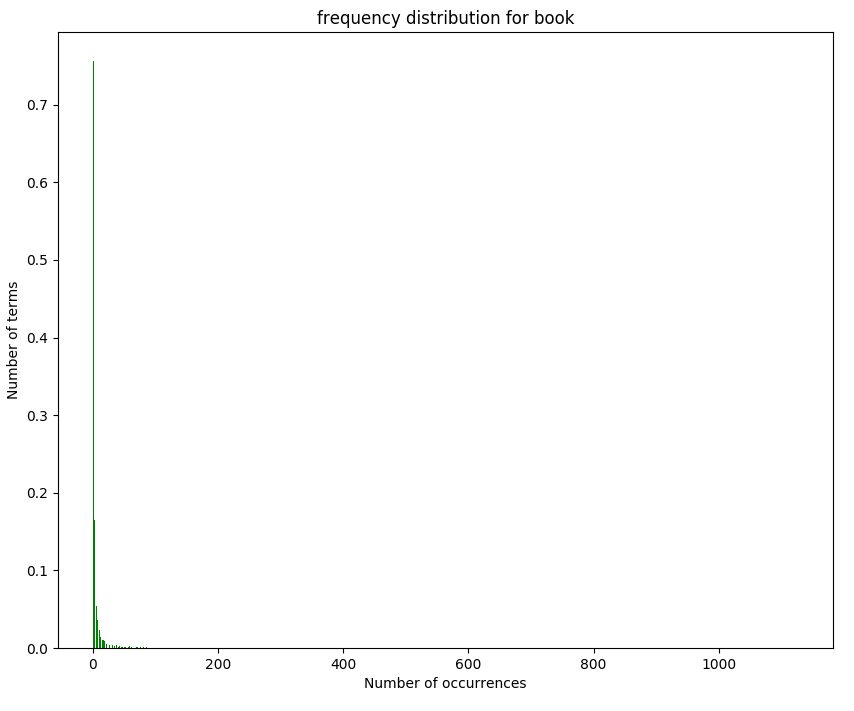
\includegraphics[width=0.5\textwidth]{./images/frequency-distribution-book.png}
\end{figure}
\end{flushleft}

\subsubsection{Top 20 words}
\begin{center}
\begin{tabular}{|c|c|c|c|c|c|c|c|c|c|}
\hline
mr & elizabeth & could & would & said & darcy & bennet & much & must & sister\\
\hline
miss & one & lady & jane & bingley & know & though & never & time & soon\\
\hline
\end{tabular}
\end{center}
The ordering is 1-10 on the top row and 11-20 on the bottom row.

\subsubsection{Observations}
\begin{flushleft}
Note that a majority of the top-20 words are proper nouns. This is because of the removal of stopwords, and lemmatization that causes most of the common words to get reduced to their base forms.
\(\newline\)

The distribution plot shows us an approximate version of the exponential distribution. Words that occur lesser and exponentially lesser in number.
\end{flushleft}

\subsection{Metric: Entropy}
\subsubsection{Distribution Plot}
\begin{figure}[H]
\centering
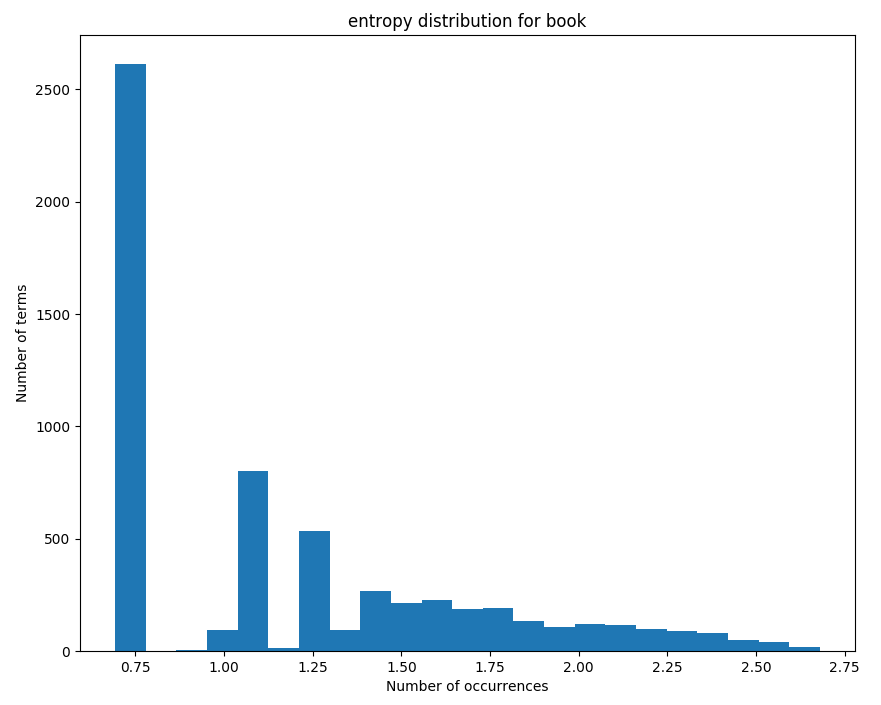
\includegraphics[width=0.5\textwidth]{./images/entropy-distribution-book.png}
\end{figure}

\subsubsection{Top 20 words}
\begin{center}
\begin{tabular}{|c|c|c|c|c|c|c|c|c|c|}
\hline
would & mr & much & could & elizabeth & little & one & without & great & soon\\
\hline
day & said & must & time & never & family & see & however & sister & well\\
\hline
\end{tabular}
\end{center}
The ordering is 1-10 on the top row and 11-20 on the bottom row.

\subsubsection{Observations}
\begin{flushleft}
Unlike observed while using the frequency metric, there are more common nouns than proper nouns in the top-20 collection. However, there are still fewer verbs than nouns or adjectives.
\(\newline\)

Despite this difference with the kinds of words in top-20 collection, the distribution of entropy is similar to the distribution of frequency shown earlier. Here too, the distribution looks like an exponential distribution, where words with lower entropy occur exponentially lower in number.
\end{flushleft}

\subsubsection{Scatter Plot between Frequency and Entropy}
\begin{flushleft}
\begin{figure}[H]
\centering
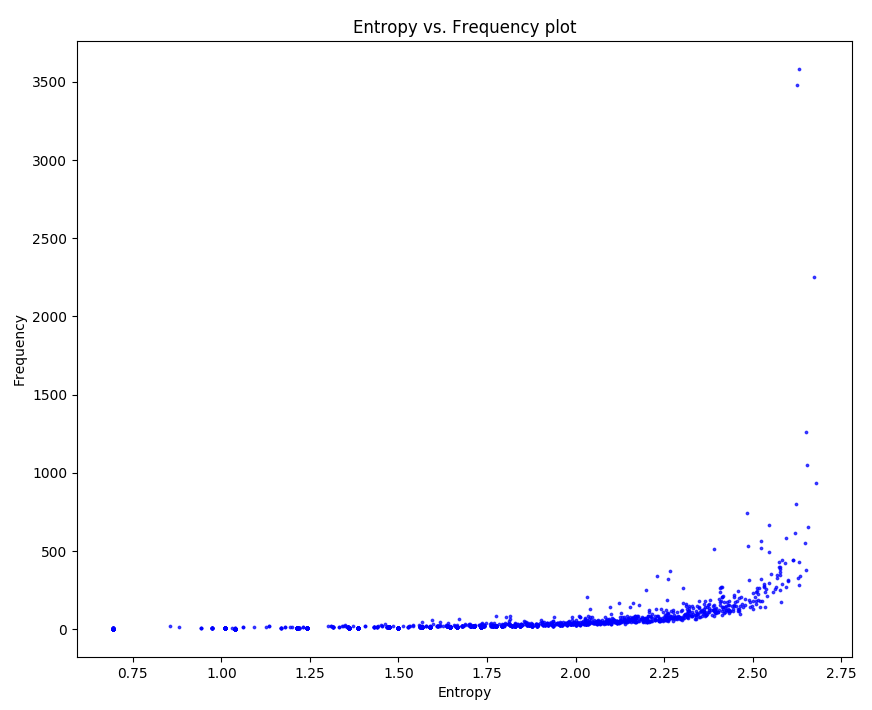
\includegraphics[width=0.6\textwidth]{./images/scatter-plot.png}
\end{figure}
Notice that this plot looks more like an exponential function. There is a lot of concentration of terms (essentially entropy-frequency pairs) in the middle of the plot.
\end{flushleft}

\subsection{Metric: Sum-of-ranks (custom metric)}
\subsubsection{Explanation}
\begin{flushleft}
The method of sum-of-ranks is simple. Given \(n\) terms, compute the frequency-based rank of every term \(t_{i}\) in every chapter of the book. Now, sum the ranks of all every terms obtained across all the chapters. Proceed to give a ranking based on this sum - the lower the magnitude of \textit{sum of ranks}, the better.
\(\newline\)

The intuition behind this scheme is that : words that are consistently prominent are more prominent (or in this case, ranked higher) than those words that are less prominent or words that are prominent occasionally (i.e., ranked lower).
\end{flushleft}

\subsubsection{Advantages / Disadvantages}
A naive advantage is that one can see that this ranking seeks consistency. The rank of terms is at most the lowest rank is has obtained, and at least the highest rank it has obtained. However useful this method maybe, this is time consuming if computed serially. For a book with \(C\) chapters, there needs to be \(C\) sortings required, meaning this won't scale as well for enormous texts.

\subsubsection{Top 20 words}
\begin{center}
\begin{tabular}{|c|c|c|c|c|c|c|c|c|c|}
\hline
mr & would & elizabeth & one & much & without & little & could & said & bennet\\
\hline
however & time & first & make & jane & man & though & thought & hope & many\\
\hline
\end{tabular}
\end{center}
The ordering is 1-10 on the top row and 11-20 on the bottom row.

\subsubsection{Observations}
The words obtained seem to look like a combination of words obtained from a frequency-based ranking as well as a entropy-based ranking. Still, there are not as many verbs as there are nouns and adjectives.
\end{document}
